\documentclass[letterpaper,11pt]{article}

%packages
\usepackage{amsfonts}
\usepackage{graphicx}
\usepackage[left=2cm,top=2cm,right=2cm,bottom=1.5cm,head=.5cm,foot=.5cm]{geometry}
\usepackage{url}
\usepackage{multirow}
\usepackage{longtable}
\usepackage{subfig}
\usepackage{float}
\usepackage{setspace}
\usepackage{lineno}
\usepackage{natbib}
\usepackage{amsmath}
\usepackage{authblk}
\usepackage{xr}
\usepackage{relsize}
\usepackage{tikz}
\usepackage{Sweave}

%external documents
\externaldocument[SI-]{SupMat}

%new commands and so on
\providecommand{\keywords}[1]
{
  \small	
  \textbf{\textit{Keywords---}} #1
}

\DeclareMathOperator{\E}{\mathbb{E}}% expected value
\DeclareMathOperator{\var}{var}
\DeclareMathOperator{\cov}{cov}
\DeclareMathOperator{\cor}{cor}
\DeclareMathOperator{\mean}{mean}
\DeclareMathOperator{\se}{se}
\DeclareMathOperator{\sd}{sd}
\DeclareMathOperator{\prob}{P}

%attempt 1 at nat and sharp
%\newcommand{\nat}{\mathlarger{\natural}}
%\newcommand{\shp}{\mathlarger{\sharp}}

%attempt 2 at nat and sharp
%\newcommand{\nat}{\raisebox{1pt}{\mathsmaller{\mathsmaller{/\hspace{-2pt}/}}}}
%\newcommand{\shp}{\#}

%attempt 3 at nat and sharp
\newcommand{\nat}{%
\text{\hspace{-1.5pt}
\begin{tikzpicture}[scale=1.8]%
\draw (.333ex,0) -- (.333ex,1ex);%
\draw (.666ex,0) -- (.666ex,1ex);
\end{tikzpicture}%
}}
\newcommand{\shp}{%
\text{\hspace{-1.5pt}
\begin{tikzpicture}[scale=1.8]%
\draw (0,.333ex) -- (1ex,.333ex);%
\draw (0,.666ex) -- (1ex,.666ex);%
\draw (.333ex,0) -- (.333ex,1ex);%
\draw (.666ex,0) -- (.666ex,1ex);
\end{tikzpicture}%
}}
\newcommand{\test}{%
\text{
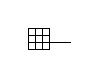
\begin{tikzpicture}[scale=1.8]%
\draw (0,0) -- (1ex,0ex);
\draw (0,0) -- (0ex,1ex);
\draw (0,1ex) -- (1ex,1ex);
\draw (1ex,0) -- (1ex,1ex);
\draw (0,.333ex) -- (2ex,.333ex);%
\draw (0,.666ex) -- (1ex,.666ex);%
\draw (.333ex,0) -- (.333ex,1ex);%
\draw (.666ex,0) -- (.666ex,1ex);
\end{tikzpicture}%
}}

\newcommand{\olr}{\overline{r}}
\newcommand{\olrs}{\overline{r}^{\shp}}
\newcommand{\olrn}{\overline{r}^{\nat}}
\newcommand{\bs}{\backslash}

%header material for paper
\title{Working document to try to explain why/how ATAs influence coexistence in an intuitive way for referee 3}
\date{}

\author[a,b]{Pimsupa Jasmin Albert}
\author[a,c,*]{Daniel C. Reuman}

\affil[a]{Department of Ecology and Evolutionary Biology and Center for Ecological Research, University of Kansas}
\affil[b]{Environmental Studies Program and Department of Biology, University of Oregon}
\affil[c]{Laboratory of Populations, Rockefeller University}
\affil[*]{Corresponding author, reuman@ku.edu}

%for dealing with line numbers bugs having to do with equations
\let\oldequation\equation
\let\oldendequation\endequation
\renewenvironment{equation}
  {\linenomathNonumbers\oldequation}
  {\oldendequation\endlinenomath}
\let\oldalign\align
\let\oldendalign\endalign
\renewenvironment{align}
  {\linenomathNonumbers\oldalign}
  {\oldendalign\endlinenomath}

\begin{document}

\maketitle

\section{Initial thinking}

This approach is nothing analogous to attempts I have seen to intuitively explain storage effects. Part of the
reason for that is that those attempts may be rooted at least partly in the Chesson theory, which assumes
small noise. We no longer make that assumption, and we already know (or strongly suspect, based on the 
intuition provided by Steve Ellner) that ATAs will not make any difference under a small noise assumption,
because under such an assumption the approximations of Chesson are good. The approach described here also has other differences, 
discussed below. One major shortcoming is that this approach provides little ecological intuition as to what ATA
effects precisely are, even if it does (I hope) make it seem not only plausible but expected that they should
frequently matter. And it provides some mathematical intuition that could prehaps be substituted for purely
ecological intuition in some sense. I look forward to discussing this approach with Jasmin before possibly putting some version 
of it in the paper.

We mainly consider the lottery model. Though we begin with some more general notation, we quickly make an
assumption that I think will only hold for the lottery model.
We assume, as usual, that for whatever model we consider (a 2-species model), we can write $r_i$ as
a function of $E_i$ and $C_i$, and $r_i$ is an increasing function of $E_i$ and decreasing function
of $C_i$. Then ATA effects are defined as
\begin{align}
\Delta_i^{[EC]} &= (\olr_{i \bs i} - \olr_{j \bs i})-(\olrn_{i \bs i} - \olrn_{j \bs i}) \label{eq:ATAeffects1}\\
&= (\olr_{i \bs i} - \olrn_{i \bs i}) - (\olr_{j \bs i} - \olrn_{j \bs i}) \label{eq:ATAeffects2}\\
&= (\olr_{i \bs i} - \olrn_{i \bs i}).
\end{align}
The third term in (\ref{eq:ATAeffects2}) is $0$ because that represents growth of $j$ in a steady-state scenario,
and the fourth term is $0$, for the lottery model, because of reasoning in S5.1. So here is where we are 
getting specific to the lottery model, as warned above. Maybe the next iteration of this thinking should 
consider what happens when that fourth term does not vanish. Can we generalize? I think we can - see below for
some efforts to generalize which were added later.

For the lottery model, we have 
\begin{align}
\Delta_i^{[EC]} &= (\olr_{i \bs i} - \olrn_{i \bs i}) \\
&= \E \left[ \ln \left( 1-\delta+\frac{E_i}{C_{i \bs i}} \right) \right] - \E \left[ \ln \left( 1-\delta+\frac{E_i^\nat}{C_{i \bs i}^\nat} \right) \right]. \label{eq:DeltaTerm1} 
\end{align}
The first term of (\ref{eq:DeltaTerm1}) is the average of the function $\ln(1-\delta+x/y)$ over the bivariate 
distribution $(E_i,C_{i \bs i})$, whereas the second term of that expression is the average of the same
function over the distribution $(E_i^\nat,C_{i \bs i}^\nat)$. We can visualize these averages pretty easily and 
effectively (see below) for specific distributions, and it helps to see how ATAs can influence coexistence.
Fig. \ref{thefig} shows this visualization. For the log-normal fecundities model (A-D), the average value of the 
function over the green points should be about the same on each panel as over the black points, 
corresponding to the fact that $\Delta_i^{[EC]}$ is close to zero for the parameters used (see Fig. 2). 
On the other hand, for the beta-fecundities model for left-tail associated noise (E, F), the average of the function 
over the black points is obviously going to be bigger than its average over the green points, corresponding to the 
fact that, for these parameters, $\Delta_i^{[EC]}$ is negative (Fig. 3).
For the beta-fecundities model for right-tail associated noise (G, H), the average of the function 
over the black points is obviously going to be smaller than its average over the green points, corresponding to the 
fact that, for these parameters, $\Delta_i^{[EC]}$ is positive (Fig. 3).

\begin{figure}
\includegraphics[width=\textwidth]{../results_figs/PostHocExplanatoryFig.jpg}
\caption{Pictorial representation of $\E \left[ \ln \left( 1-\delta+\frac{E_i}{C_{i \bs i}} \right) \right]$ and 
$\E \left[ \ln \left( 1-\delta+\frac{E_i^{||}}{C_{i \bs i}^{||}} \right) \right]$ for the 
log-normal-fecundities lottery model (A-D) and the beta-fecundities lottery model (E-H),
for left-tail associated noise (A, B, E, F), and for right-tail associated noise (C, D, G, H).
The color and contours show $\ln(1-\delta+x/y)$, whereas the green points on each panel show a sample from
the distribution $(E_i,C_{i \bs i})$ and the black points show a sample from the distribution 
$(E_i^{||},C_{i \bs i}^{||})$. Thus the average value of the function over the green points minus its
average value over the black points is a good approximation of $\Delta_i^{[EC]}$. Here $i=1$ and
$j=2$. We used parameters $\sigma=1$, $\mu_1 = 0$, and $\mu_2 = 0.5$ for the log-normal fecundities
model; $\eta_1 = 1$ and $\eta_2 = 1.2$ for the beta-fecundities model; and $\delta=0.6$
for both models. Results are plotted on both linear (A, C, E, G) and log (B, D, F, H) 
scales for readability.}\label{thefig}
\end{figure}

Viewing $\Delta_i^{[EC]}$ as an average of a function over a set of points distributed in a certain way
(with ATAs) minus an average of the same function over a set of points distributed in another way
(with ATAs removed) makes it clear why we would expect to commonly see substantial ATA effects 
on coexistence: removing ATAs really changes the way points in a bivairate distribution are 
distributed, in a way that can interact strongly with averaging over a function representing growth of
a potential invader. In fact, it seems clear that only very special functions will give the exact same results 
when averaged over a typical distribution with ATAs or with ATAs removed.

Growth from rarity, $\olr_{i \bs i}$ is an average of the individual growth rates which pertain across
years, and those values depend on the details of the distribution of $E$ and $C$. If we use 
$E_i$ and $C_{i \bs i}$, well then of course we will tend to get different values
from if we use $E_i^\nat$ and $C_{i \bs i}^\nat$. The question is just how much different, which is what 
we have sought to answer with this paper for lottery model and experimental examples. 

\section{Efforts to generalize}

Equation (\ref{eq:ATAeffects2}) is what we had prior to specifying to the lottery model. 
Above, we've considered the first two terms, which are the average of $r_i(E_i,C_i)$ over 
the distribution $(E_i,C_{i \bs i})$ minus the average of the same function
over $(E_i^\nat,C_{i \bs i}^\nat)$. But the last two terms of (\ref{eq:ATAeffects2})
are the average of $r_i(E_j,C_j)$ over the distribution $(E_j,C_{j \bs i})$ minus the 
average of the same function over $(E_j^\nat,C_{j \bs i}^\nat)$. So the same basic
ideas apply here as in the lottery model case, it's just that we have to make two comparisons 
of growth functions averaged over distributions, one comparison for the invader, $i$,
and the other for the resident, $j$. Again, essentially any model will have 
non-zero value of (\ref{eq:ATAeffects2}) -- only models designed as counterexamples
should typically have a precisely zero value for that expression. So ATAs will always
matter to some extent for coexistence. It's just a question of how much, for real systems. 
And, as far as can tell, that can only be answered by computing these quantities for
several real systems. We've shown that, at least for some systems, the quantities 
can be meaningfully large.

\section{Additional commentary/thinking by writing}

OK, it seems clear to me that basically any meanigful change to the distribution 
$(E,C)$ will typically alter the average value of the nonlinear function $r(E,C)$ 
over that distribution. There are many ways to decompose the growth rate 
$\olr_{i \bs i}$ through a series of alterations of the distribution $(E,C)$. 
Ellner et al. also make this point in their 2019 paper. The original Chesson 
theory is probably the most natural decomposition under a weak noise assumption,
but Ellner et al. and our paper make it clear there are other ways that may make
more sense, in some circumstances, if noise is not weak. 





\end{document}